\definecolor{codeComment}{RGB}{0, 128, 0}
\definecolor{codeKeyword}{RGB}{0, 0, 255}
\definecolor{codeNumber}{RGB}{100, 100, 255}
\definecolor{codeString}{RGB}{100, 100, 255}
\lstdefinestyle{delphicode}{
	language=Delphi, 
	commentstyle=\color{codeComment},
	keywordstyle=\color{codeKeyword},
	numberstyle=\tiny\color{codeNumber},
	stringstyle=\color{codeString},
	basicstyle=\ttfamily\footnotesize,
	breaklines=true,
	showspaces=false,
	showstringspaces=false
}
\lstset{style=delphicode}


\Chapter{Megvalósítás}

A program gyakorlati megvalósítása egy-két apróságtól eltekintve megegyezik a terve\hyp{}zettel. Az alapvető stuktúra az tartva lett, az egymáshoz tartozó funkciók, változók és kódrészletek külön egységekbe (továbbiakban: unitok) lettek szedve, így csoportosítva az egyes szoftverfunkciókat.

Ezeknek a unitok többféle kapcsolatban állhatnak egymással, az egymásra való hivatkozásuknak függvényében. Ezeket a kapcsolatokat a következő ábra demonstrálja.

\begin{figure}[h]
	\begin{center}
		\caption{Unitok kapcsolatai}
		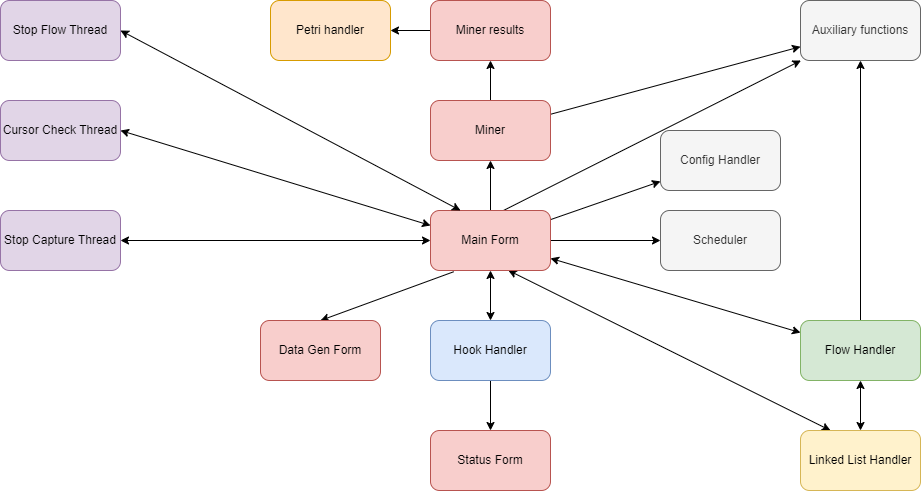
\includegraphics[width=\textwidth, keepaspectratio=true]{images/unitok_kapcsolati_abra}\\
		\label{fig:example}
	\end{center}
\end{figure}

Pirossal azok a unitok vannak ábrázolva melyekhez tartozik grafikus felület is, a további színek pedig az egyes funkciók csoportosítására szolgálnak. Részletesebben a unitokról:

\begin{itemize}
	\item{
		\textbf{Unit\_Main}: Ez a program főegysége, ebben került implementálásra a főablak és annak felhasználói felülete, számos funkciót lát el:
		\begin{enumerate}
			\item{Implementálja a felhasználói felület objektumait, azoknak a tulajdonságait és rutinjait,}
			\item{Inicializálja a programot futtatásnál, betölti a felhasználó konfigurációit,}
			\item{Kezeli a program rendszertálcára való kicsinyítését,}
			\item{Kezeli azt a néhány globális változót amik szükségesek (pl. a futtatható fájl elérési útvonala).}			
		\end{enumerate}
	}
	\item{
		\textbf{Unit\_ConfigHandler}: Konfigurációkezelő osztályt és az abba tartozó objek\hyp{}tumokat és rutinokat implementálja, melyek lehetővé teszik a futásidő alatti konfigurációs beállítások titkosítva történő tárolását.
		\begin{lstlisting}
  TConfigHandler = class(TObject)
    configFile: string;
    configArray : array of array of string;

  public
    procedure Save(Key: string; Value: string);
    function Load(Key: string; Fallback: string): string;

    constructor Create(filePath: string);
    destructor Destroy; override;

    function Encrypt(const value: string): UnicodeString;
    function Decrypt(const value: string): UnicodeString;

    function MatchCharToArrayIndex(const character: char): integer;
  end;
		\end{lstlisting}
	}
	\item{
		\textbf{Unit\_AuxiliaryFunctions}: Néhány olyan kiegészítő rutint tartalmazó gyűjte\hyp{}mény, melyeket a többi egység használ. Külön egységbe ki lettek gyűjtve, hogy az OOP alapelvek teljesüljenek.
	}
	\item{
		\textbf{Unit\_StopFlowThread}: Egy olyan szálat implementáló egység, amely feladata kifejezetten a \textbf{F2 + F3} billentyűkombináció lenyomásának felügyelete.

		Ez a billentyűkombináció felel azért, hogy az éppen futó folyamatot le lehessen futás közben állítani. Feltétlenül szükséges, hogy ez ilyen módon legyen implemen\hyp{}tálva, hiszen ennek a billentyűkombinációnak akkor is működnie kell, ha a fókusz éppen egy másik alkalmazáson van.

A Windows API és a \textbf{Unit\_Main} által implementált rutinokra és változókra hivatkozik a műküdése során.
		\begin{lstlisting}
procedure TStopFlowThread.Execute;
begin
  repeat
    if (GetKeyState(VK_F2) < 0) and (GetKeyState(VK_F3) < 0) then begin
      Form1.Btn_StartFlowClick(stopFlowThread);
    end;
  until not runStopFlow;
end;
		\end{lstlisting}
	}
	\item{
		\textbf{Unit\_CursorCheckThread}: Egy olyan szálat implementáló egység, melynek feladata a kurzor aktuális pozíciójának a felhasználói felületen történő frissítése. Windows API-t meghívva jut hozzá a szükséges adathoz.
		\begin{lstlisting}
procedure TCursorCheckThread.Execute;
var
  p: TPoint;
begin
  FreeOnTerminate := true;
  repeat
    GetCursorPos(p);
    Form1.Lab_Cursor_X.Caption := 'x: ' + IntToStr(p.X);
    Form1.Lab_Cursor_Y.Caption := 'y: ' + IntToStr(p.Y);
  until not runCursorPos;
end;
		\end{lstlisting}
		Ennek a célja, az, hogy amikor a felhasználó kézileg akar egérkattintást hozzáadni az aktuális folyamathoz, akkor megkönyítse a megfelelő képernyő-koordináták meghatározását.
	}
	\item{
		\textbf{Unit\_StopCaptureThread}: Egy olyan szálat implementáló egység, melynek feladata hasonló az előzőekben bemutatott \textbf{TStopFlowThread}-éhez.

Az eltérés annyi, hogy az \textbf{F2 + F4} billentyűkombinációt figyeli, melynek lenyo\hyp{}mására egy olyan rutint hív meg, mely leállítja az éppen futó felhasználói ese\hyp{}ménysor rögzítését.
	}
	\item{
		\textbf{Unit\_LinkedListHandler}: Egy olyan struktúrát implementál, melyre a szoft\hyp{}ver összes többi folyamatkezezlő egysége épül. Az ebből a láncolt lista struktúrá\hyp{}ból példányosított elemek tartalmazzák a folyamati lépésekhez tartozó összes információt.

	Először is implementál két felsorolás típust, melyek inuitív módon leírják magu\hyp{}kat:
	\begin{lstlisting}
type
  // Enum
  TInputType = (itClick, itKeyboard, itSpecialKey, itHotkey);
  TWaitType = (wtMil, wtSec, wtMin, wtHour);
	\end{lstlisting}

	Valamint definiálja a láncolt lista elemet és az arra hivatkozó mutatót:
	\begin{lstlisting}
  // Linked List pointer type
  PFlowElement = ^TFlowElement;

  // Linked List element
  TFlowElement = record
    inputType : TInputType;
    inputParam1 : string;
    inputParam2 : string;
    inputParam3 : string;
    inputParam4 : string;
    waitAfterAmount : integer;
    waitAfterType : TWaitType;
    waitAfterTypeText : string;
    deleteButton : TButton;
    panelObject : TPanel;
    labelObject : TLabel;
    NextElement : PFlowElement;
  end;
	\end{lstlisting}

	Ezek mellett még tartalmaz egy rutint, mely arra szolgál, hogy egy meglévő láncolt lista elemtől kezdve az összes további elemhez tartalmazó objektumot megfelelően szabadítsa fel a memóriából.

	}
	\item{
		\textbf{Unit\_FlowHandler}: A folyamatokhoz tartozó legfonotsabb rutinokat definiál\hyp{}ja, amik a következőek:
		\begin{enumerate}
			\item{Folyamat mentése fájlba,}
			\item{Folyamat betöltése állományból,}
			\item{Folyamat generálása a felhasználói bevitelből rögzített eseméysorból,}
			\item{Adott folyamati lépés végrehajtása, azaz input injektálása a Windows felé. pl.:
				\begin{lstlisting}
if (currentStep.inputParam3 = 'Left') and (currentStep.inputParam4 = 'Down+Up (single)') then begin
  mouse_event(MOUSEEVENTF_LEFTDOWN, 0, 0, 0, 0);
  mouse_event(MOUSEEVENTF_LEFTUP, 0, 0, 0, 0);
end 
				\end{lstlisting}
			} 
			
		\end{enumerate}
	}
	\item{
		\textbf{Unit\_HookHandler}: Ennek az egységnek a feladata azoknak az objektumok\hyp{}nak, változóknak és függvényeknek az implementációja, melyek lehetővé teszik a felhasználói input rögzítését a Windows API \textit{hook}-jainak felhasználásával.

A \textit{hook} egy olyan pont a rendszer üzenetkezelő mechanizmusában, ahová a szoft\hyp{}ver egy olyan szubrutint telepít mely figyeli az üzenet forgalmat a rendszerben, és feldolgozza azokat még mielőtt elérné a cél-ablakhoz tartozó eljárását.

A felhasználói input rözítésénél két ilyen \textit{hook} kerül telepítésre, egy a billentyűzet üzenetsorának, a másik pedig az egérhez tartozóhoz. Ezek a telepítések a Win\hyp{}dows API által bizotsított
\begin{lstlisting}
	function SetWindowsHookEx; external user32 name 'SetWindowsHookExW';
\end{lstlisting}
függvény hívásával történnek.

Ezeken túl az egység tartalmaz egy olyan funkciót is mely az adott konstanst (vagy karakterkódot) ember által könnyen értelmezhető szövegre fordítja, pl. \textbf{VK\_PRIOR} $\rightarrow$ \textbf{[Page Up]}, vagy \textbf{65} $\rightarrow$ \textbf{[a]}

	}
	\item{
		\textbf{Unit\_Status}: Ez az egység azt az ablakot implementálja, mely visszajelzést ad az éppen futó eseménysor-rögzítés lépéseiről.
		\begin{lstlisting}
type
  TForm_Status = class(TForm)
    Lab_Input: TLabel;
    Lab_Finish: TLabel;
    Lab_Input_Title: TLabel;
    Lab_StepID_Title: TLabel;
    Pnl_Main: TPanel;
    Lab_StepID: TLabel;
    procedure FormCreate(Sender: TObject);
    procedure FormShow(Sender: TObject);
    procedure FormMouseMove(Sender: TObject; Shift: TShiftState; X, Y: Integer);
  public
    procedure UpdateLabel_Input(newText: string);
    procedure UpdateLabel_StepID(newID: integer);
  end;
		\end{lstlisting}

A rutinjai lehetővé teszik, hogy más egységből (pl.: Unit\_LinkedListHandler) is lehessen frissíteni a grafikus elemeit, valamint, hogy folyamatrögzítés közben hiába látszik az ablak, akkor se legyen útban a felhasználónak.
	}
	\item{
		\textbf{Unit\_Scheduler}: Két egyszerű függvényt implementáló osztályt definiál, mely arra szolgál, hogy a Windows API segítségével meghívott \textit{schtasks.exe} feladatüte\hyp{}mezőbe rögzíteni, illetve onnan törölni lehessen folyamatokat.
	\begin{lstlisting}
  TScheduleHandler = class(TObject)
  public
    function DeleteTask(fPath: string): integer;
    function AddTask(fPath, sPath: string): integer;
  end;
	\end{lstlisting}
	}
	\item{
		\textbf{Unit\_DataGenerator}: Egy felületet és számos rutint definiál, melyek segítsé\hyp{}gével könnyedén folyamatokat lehet generálni. Ennek az a célja, hogy az adatbá\hyp{}nyászathoz elegendő mennyiségű folyamatot lehessen meghatározni emberi időn belül.

	\begin{lstlisting}
type
  TForm_Generator = class(TForm)
    Mem_Log: TMemo;
    Pnl_Interface: TPanel;
    Btn_Generate: TButton;
    RadGroup_GenCategory: TRadioGroup;
    Spin_GenCount: TSpinEdit;
    procedure Btn_GenerateClick(Sender: TObject);
    procedure FormCloseQuery(Sender: TObject; var CanClose: Boolean);
  private
    { Private declarations }
    procedure Generate_ComputerShutdown(count: integer);
    procedure Generate_ComputerRestart(count: integer);
    procedure Generate_BrowserLaunch(count: integer);
    procedure AddToLog(msg: string);

    function GetClickDelay(_type: integer): integer;
    function GetRandomMouseCoordinate(min, max: integer):integer;
  end;

	\end{lstlisting}

		Három forgatókönyv került létrehozásra, ezekből választva lehetséges a generálás. A feladatot elvégezve a folyamatokat egy adott mappába állományonként menti le a szoftver.
	}
	\item{
		\textbf{Unit\_Miner}: Egy felületet és az Alpha-algoritmust implementálja. A felületet használva a bányászat megkezdését követően láthatjuk, hogy éppen hol jár az algoritmustban a szoftver.
	\begin{lstlisting}
type
  TForm_Miner = class(TForm)
    Panel_Interface: TPanel;
    Mem_Log: TMemo;
    Edt_DataPath: TEdit;
    Pnl_DataPath: TPanel;
    Lab_DataPath: TLabel;
    Btn_DataPath_Browse: TButton;
    Btn_Begin: TButton;
    procedure FormCloseQuery(Sender: TObject; var CanClose: Boolean);
    procedure Btn_DataPath_BrowseClick(Sender: TObject);
    procedure Btn_BeginClick(Sender: TObject);
  private
    procedure AddToLog(msg: string);
    procedure AlphaMine();
    procedure ChangeUserControl(newState: boolean);
    function RemoveBracketsFromString(str: string): string;
    function IsInActivityList(str: string): boolean;
    function GetNewActivityID: string;
    function FindActivityID(str: string): string;
  end;
	\end{lstlisting}

Amint végzett az algoritmus, az eredményeket a következő \textbf{Unit\_MinerResults} által definiált ablakban ábrázolja.

A halmazpárok három-dimenziós adatstruktúraban vannak tárolva illetve kezelve, ezeknek az átlátása elég komoly odafigyelést igényel.
	\begin{lstlisting}
  TArrayOfSets = array of array of array of integer;
	\end{lstlisting}

	}
	\item{
		\textbf{Unit\_MinerResults}: Azt a felületet implementáló egység, mely az Alpha-algoritmus eredményeit jelenít meg grafikusan. Ezek:
		\begin{enumerate}
			\item{A létrejött eseménynapló,}
			\item{Az eseménynaplóból meghatározott lenyomati mátrix,}
			\item{Az összes maximális halmaz,}
			\item{A kimeneti Petri-háló, melyet a \textbf{Unit\_PetriHandler} segítségével generál.}
		\end{enumerate}
		\begin{lstlisting}
  TForm_MinerResults = class(TForm)
  .
  .
  .
  public
    procedure DrawPetriNet(arrayOfSets: TArrayOfSets);
    procedure DrawPlace(startX, startY: integer; lab: string);
    procedure DrawTransition(startX, startY: integer; lab: string);

    procedure DrawArrow(startX, startY, endX, endY: integer); overload;
    procedure DrawArrow(endX, endY: integer); overload;

    function GetStartEvents(): TIntegerArray;
    function GetEndEvents(): TIntegerArray;
  end;

		\end{lstlisting}
	}
	\item{
		\textbf{Unit\_PetriHandler}: Számos objektumot és rutint implementál, melyek segít\hyp{}ségével felépíthető és megjeleníthető egy Petri-háló
		\begin{enumerate}
			\item{Definiálja a helyeket,
				\begin{lstlisting}
  TPetriPlace = record
    name: string;
    fromList: TStringArray;
    toList: TStringArray;
    location: TPoint;
    recursionLock: boolean;
  end;
				\end{lstlisting}
			}
			\item{Definiálja az átmeneteket,
				\begin{lstlisting}
  TPetriTransition = record
    id: integer;
    fromList: TStringArray;
    toList: TStringArray;
    location: TPoint;
    recursionLock: boolean;
  end;
				\end{lstlisting}
			}
			\item{Definiál egy Petri-háló gyűjteményt, melyben tárolni lehet a helyeket és átmeneteket, valamint a rutinok segítségével fel lehet térképezni a közöttük lévő kapcsolatokat.
				\begin{lstlisting}
  TPetriCollection = class(TObject)
    places: array of TPetriPlace;
    transitions: array of TPetriTransition;
    objectSize: integer;
  public
    constructor Create();
    destructor Destroy(); override;
    procedure NewPlace(_name: string; _fromList, _toList: TStringArray);
    procedure NewTransition(_id: integer; _fromList, _toList: TStringArray);
    function FindIndexOfPlace(name: string): integer;
    function FindIndexOfTransition(id: integer): integer;
    procedure MapTransitions();
    procedure MapPlaceLocation(currentTransition: TPetriTransition);
    procedure MapTransitionLocation(currentPlace: TPetriPlace);
    procedure UpdateList(var list: TStringArray; newValue: string);
    function GetMaxIndexInColumn(col: integer): integer;
  end;
				\end{lstlisting}
 Indexek alapján kerülnek meghatározásra a helyek és átmenetek közötti kapcsolatok, így a megjelenített ábra balról-jobbra értelmezendő.
			}
		\end{enumerate}
	}
\end{itemize}